\begin{figure}
    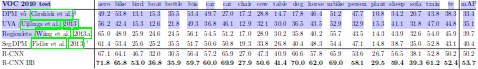
\includegraphics[width=150mm,scale=0.5]{DAP}
    \caption{Detection Average Precision \textcite{donahue}}
    \label{fig:dap}
\end{figure}

\begin{figure}
    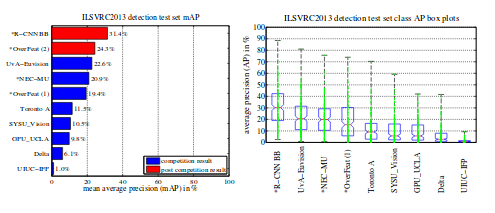
\includegraphics[width=150mm,scale=0.5]{MAP}
    \caption{Mean Average Precision \textcite{donahue}}
    \label{fig:MAP}
\end{figure}

\begin{figure}
    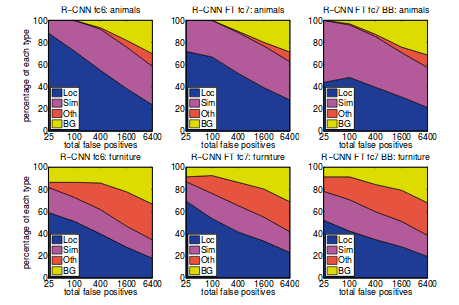
\includegraphics[width=150mm,scale=0.5]{DFP}
    \caption{Distribution of top-ranked false positives
    \textcite{donahue}}
    \label{fig:DFP}
\end{figure}

\begin{figure}
    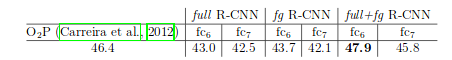
\includegraphics[width=150mm,scale=0.5]{SMP}
    \caption{Segmentation Mean Accuracy \textcite{donahue}}
    \label{fig:SMP}
\end{figure}

\begin{figure}
    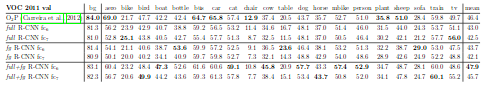
\includegraphics[width=150mm,scale=0.5]{PCATSA}
    \caption{Per-category segmentation accuracy \textcite{donahue}}
    \label{fig:PCATSA}
\end{figure}

\begin{figure}
    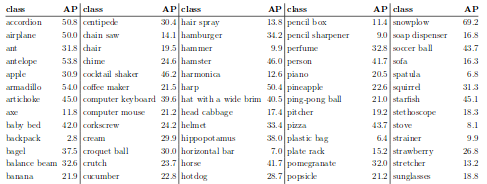
\includegraphics[width=150mm,scale=0.5]{PCLASSSA}
    \caption{Per-class segmentation accuracy \textcite{donahue}}
    \label{fig:PCLASSA}
\end{figure}

\begin{table}[]
    \centering
    \caption{My caption}
    \label{my-label}
    \begin{tabular}{ll}
        Task/Deliverable                     & Deadline \\
        Interim Report                       & 21/12/17 \\
        Select method and paper to replicate & 10/01/18 \\
        Iteration 1                          & ???      \\
        Iteration 2                          & ???      \\
        Iteration 3                          & ???      \\
        Draft Final Report                   & 08/03/18 \\
        FYP Product                          & 10/04/18 \\
        FYP Report                           & 17/04/18
    \end{tabular}
\end{table}
